\begin{frame}{Fine-Grained Recognition: Subordinate Categories}
  \begin{columns}[T,onlytextwidth]
    \column{0.48\textwidth}
      \begin{itemize}\footnotesize\itemsep0.35em
        \item \textbf{Fine-grained recognition} assigns an image to one of many subordinate categories of one basic-level category: bird species, car models, aircraft variants.
        \item \textbf{Small inter-class variation.} Classes share the same basic set of parts. In the Caltech-UCSD Birds dataset (CUB-200-2011), some pairs of species, many sparrows among them, are ``nearly visually indistinguishable, even for expert bird watchers.''
        \item \textbf{Large intra-class variation.} One species appears perched, swimming or flying, occluded, in any light and background.
        \item \textbf{Labels need experts.} Experts found 494 wrong labels in CUB-200-2011, about 4\% of its 11,788 images; citizen-science birders made 2--4 times fewer labelling errors than paid crowd workers.
      \end{itemize}
    \column{0.50\textwidth}
      \centering
      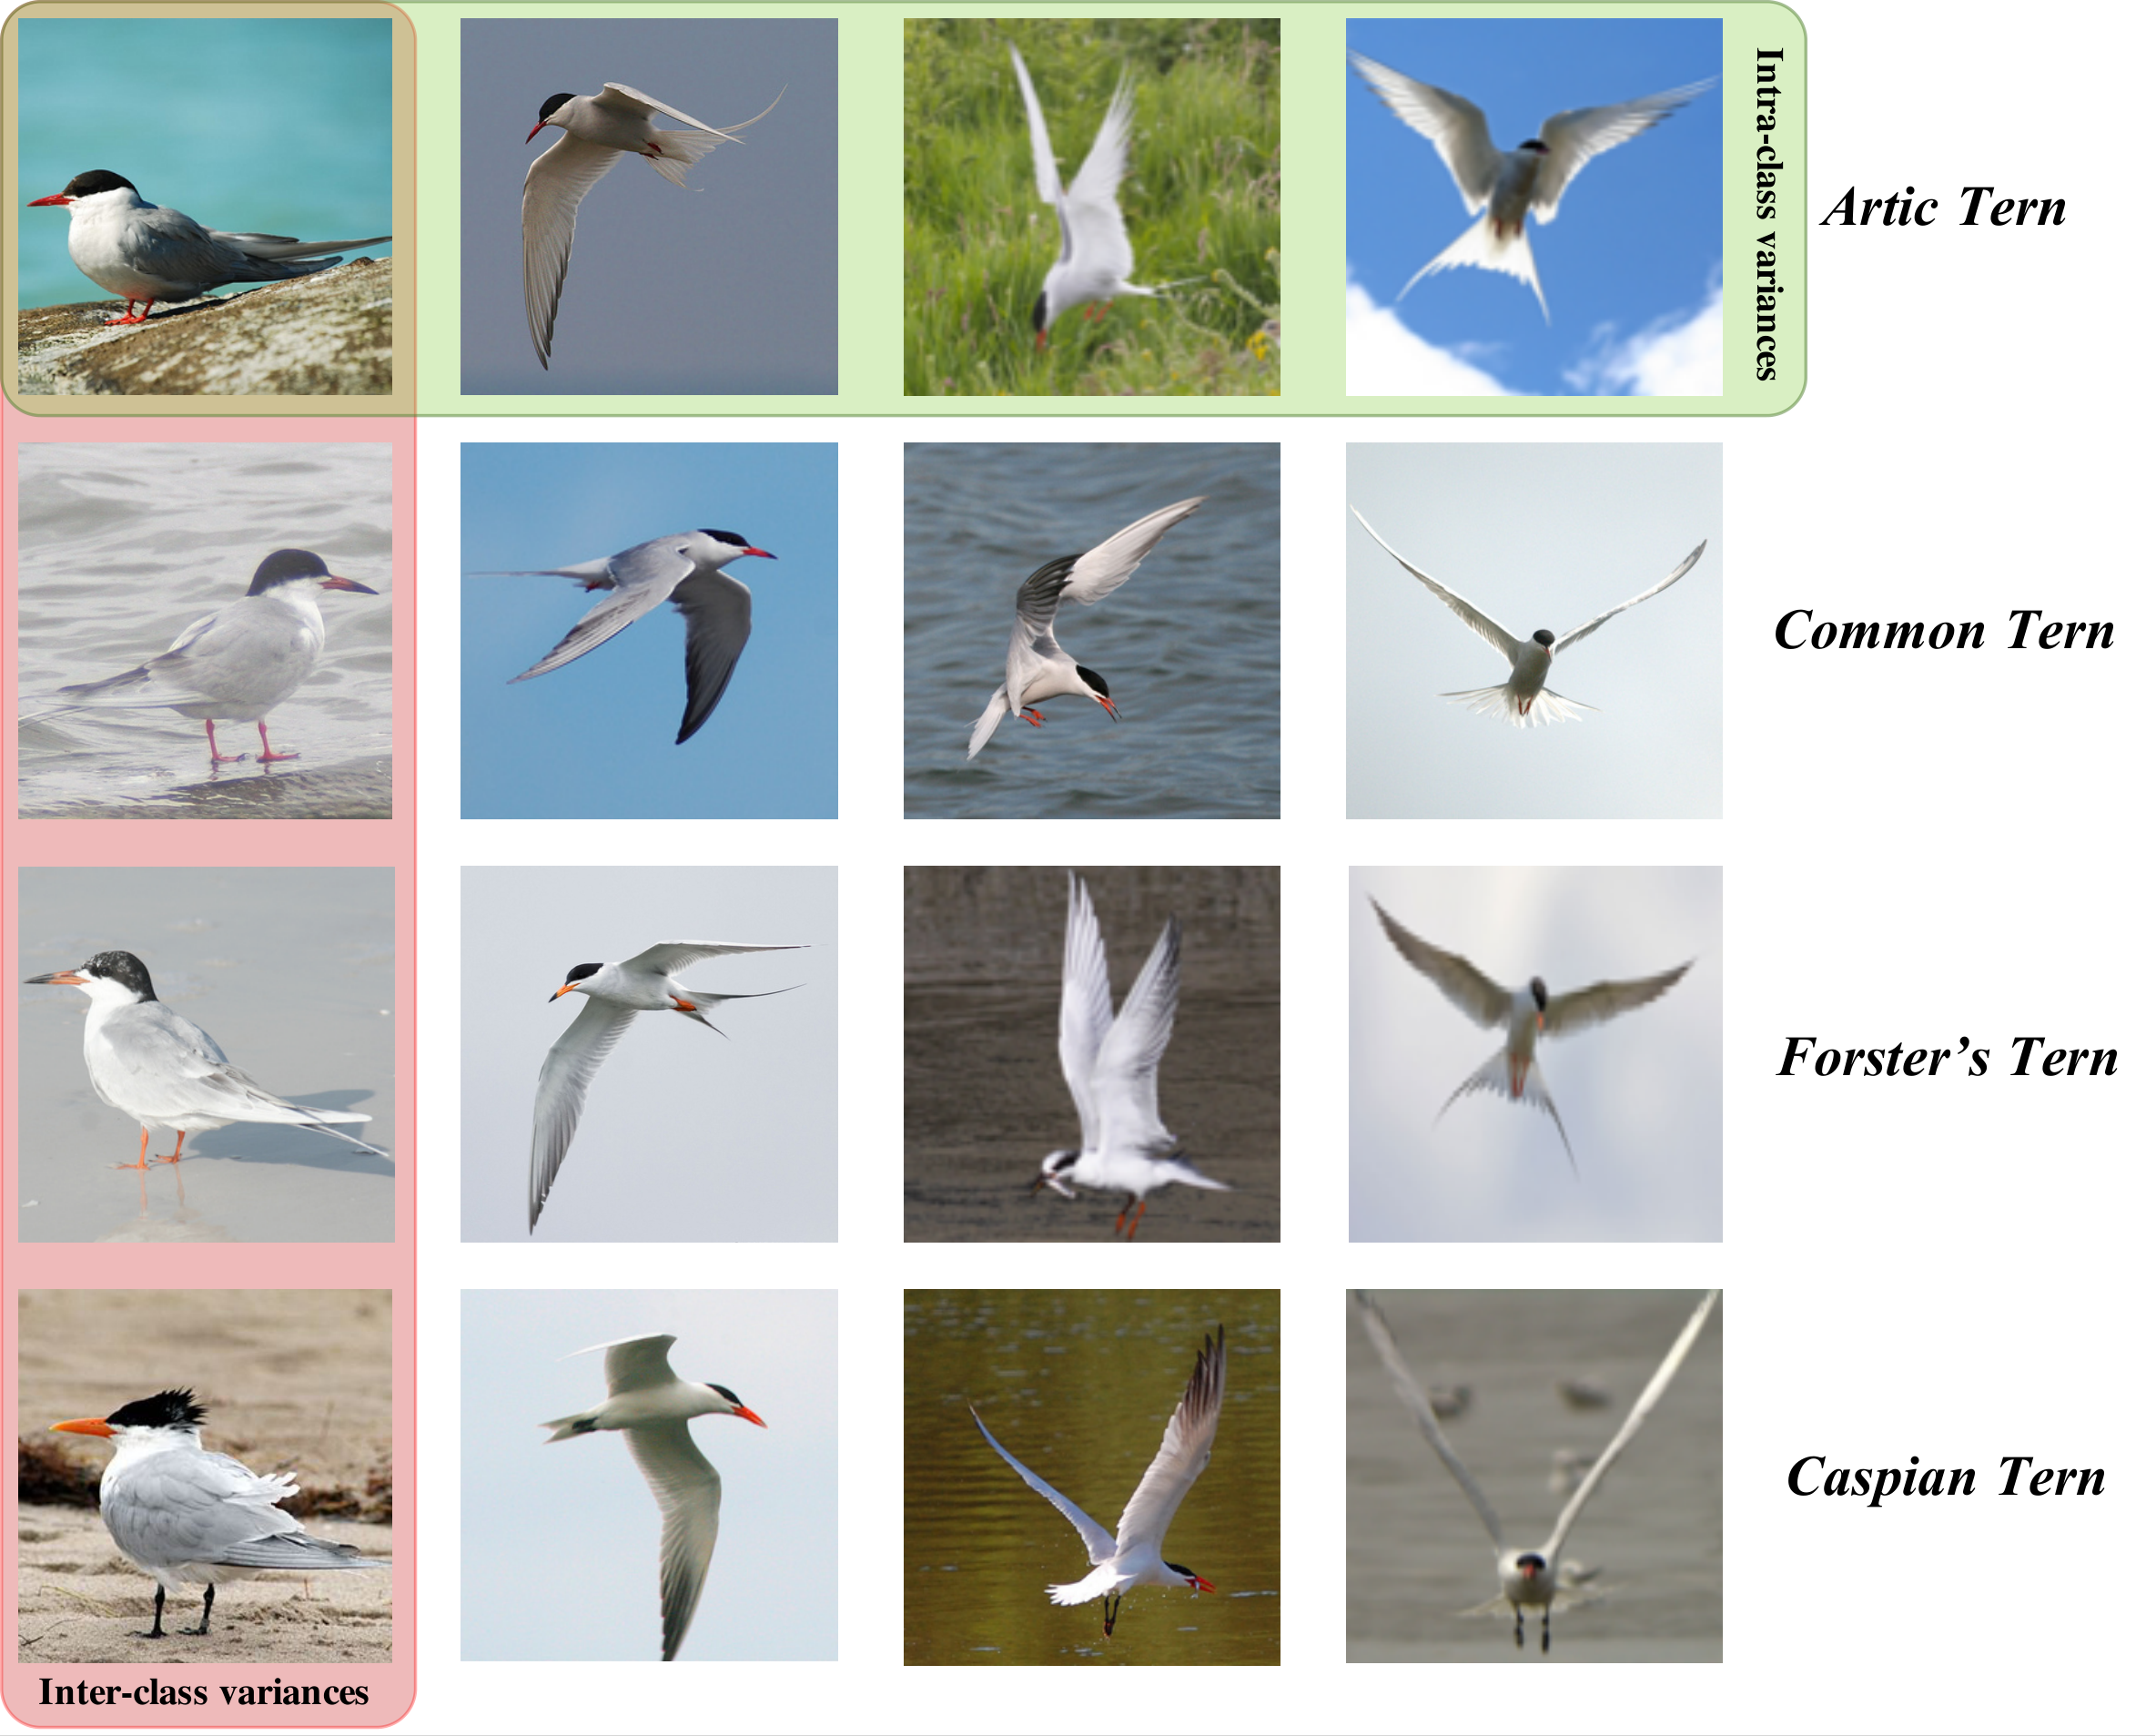
\includegraphics[width=\linewidth,height=0.58\textheight,keepaspectratio]{images/image-recognition/survey_fig4_tern_species.png}\\[0.2em]
      {\scriptsize Four tern species from CUB-200-2011, one per row. Wei et al., ``Fine-Grained Image Analysis with Deep Learning: A Survey,'' TPAMI 2022, \href{https://arxiv.org/abs/2111.06119v2}{arXiv:2111.06119v2}, Figure~4.\par}
  \end{columns}
  \vspace{0.1em}
  {\scriptsize Wah et al., ``The Caltech-UCSD Birds-200-2011 Dataset,'' Caltech technical report 2011, Sec.~1; Van Horn et al., ``Building a Bird Recognition App and Large Scale Dataset With Citizen Scientists,'' CVPR 2015, Sec.~1 and~6.\par}
\end{frame}

\begin{frame}{Fine-Grained Benchmarks}
  These benchmarks recur throughout this section; each reports classification accuracy on a fixed test split.
  \vspace{0.3em}

  {\centering\scriptsize
  \begin{tabular}{>{\raggedright\arraybackslash}p{2.3cm} >{\raggedright\arraybackslash}p{1.9cm} >{\raggedright\arraybackslash}p{1.5cm} >{\raggedright\arraybackslash}p{6.1cm}}
    \toprule
    \textbf{Dataset} & \textbf{Classes} & \textbf{Images} & \textbf{What makes it hard} \\
    \midrule
    CUB-200-2011 & 200 species & 11,788 & about 60 images per class; look-alike species; 15 part locations and 312 binary attributes annotated per image \\
    \addlinespace[0.2em]
    Stanford Cars & 196 classes & 16,185 & classes at make, model and year level, such as ``2012 Tesla Model S'' \\
    \addlinespace[0.2em]
    FGVC-Aircraft & 100 variants & 10,000 & variants of 70 families from 30 manufacturers; Boeing variants such as -200, -300 and -400 differ mostly in length \\
    \addlinespace[0.2em]
    NABirds & 555 categories & 48,562 & North American species split by sex, age or plumage into visual categories; expert-curated labels \\
    \addlinespace[0.2em]
    iNaturalist 2021 (iNat21) & 10,000 species & 2.7M (train) & the whole tree of life; train and test split by submission date, test from the latest year; a supervised ResNet-50 reaches 76.0\% \\
    \bottomrule
  \end{tabular}\par}
  \vspace{0.2em}
  {\scriptsize CUB, Stanford Cars and FGVC-Aircraft return later in this lecture. Wah et al.\ 2011; Krause et al., ``3D Object Representations for Fine-Grained Categorization,'' ICCV Workshops 2013, and its dataset page (196 released classes); Maji et al., ``Fine-Grained Visual Classification of Aircraft,'' 2013, \href{https://arxiv.org/abs/1306.5151v1}{arXiv:1306.5151v1}; Van Horn et al., CVPR 2015, Sec.~3--4; Van Horn et al., ``Benchmarking Representation Learning for Natural World Image Collections,'' CVPR 2021, \href{https://arxiv.org/abs/2103.16483v2}{arXiv:2103.16483v2}, Sec.~3.1 and Tables~1--2.\par}
\end{frame}

\begin{frame}{Before Transformers: Parts and Bilinear Pooling}
  \begin{columns}[T,onlytextwidth]
    \column{0.42\textwidth}
      \centering
      \vspace{0.6em}
      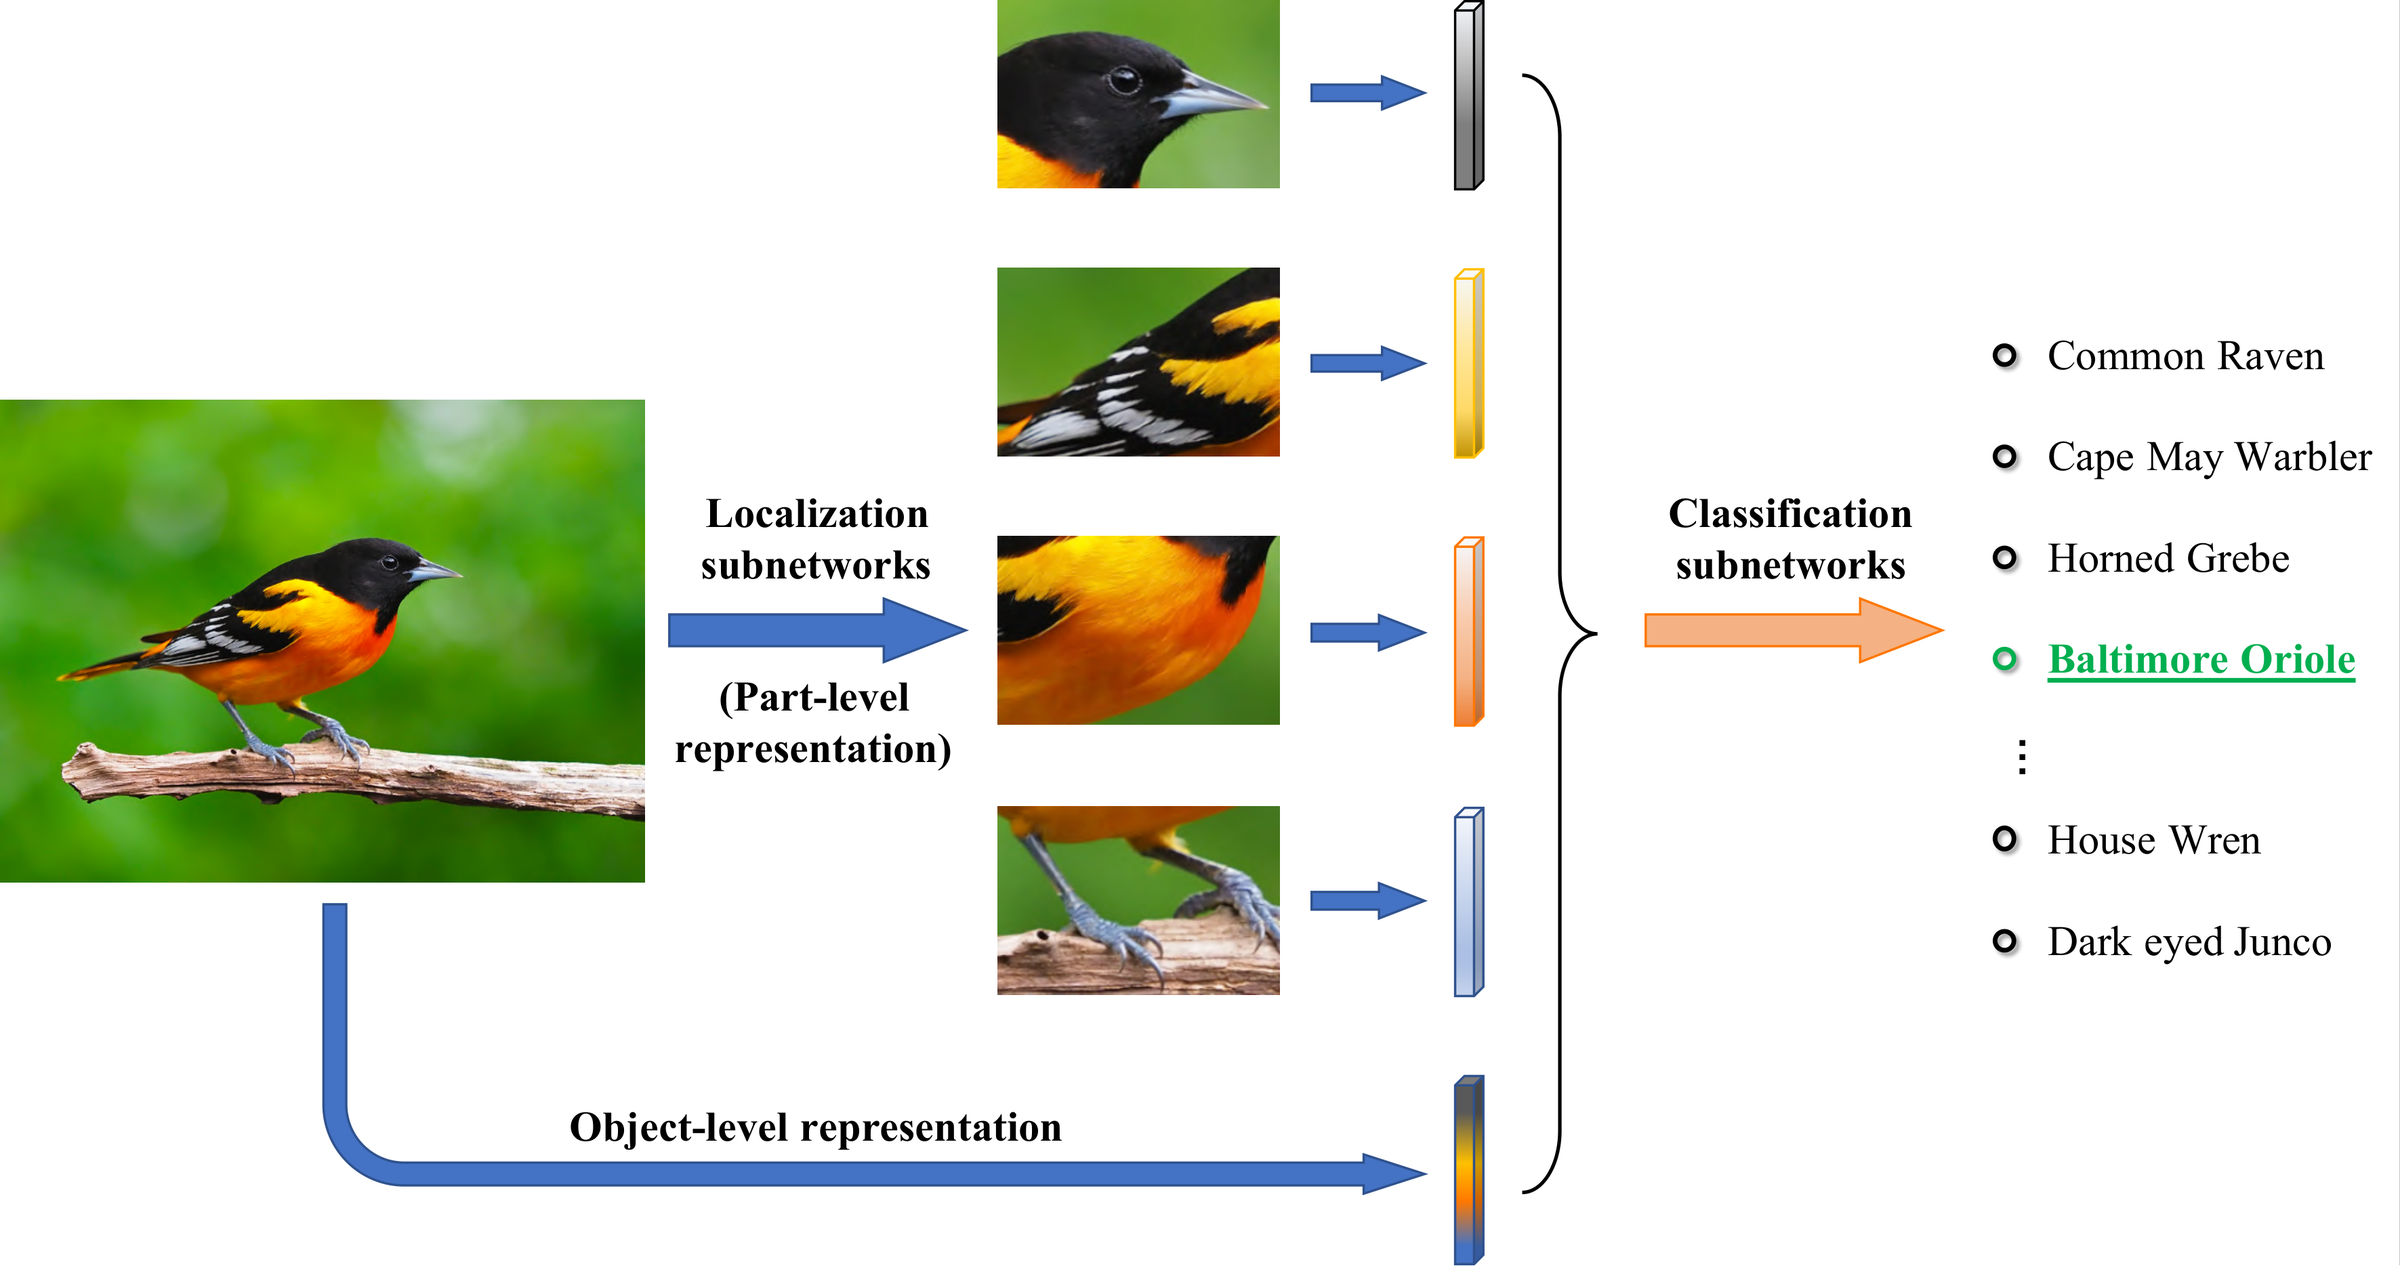
\includegraphics[width=\linewidth,height=0.46\textheight,keepaspectratio]{images/image-recognition/survey_fig8_localization_classification.png}\\[0.2em]
      {\scriptsize Localisation subnetworks crop parts; part-level and object-level features are classified together. Wei et al., \href{https://arxiv.org/abs/2111.06119v2}{arXiv:2111.06119v2}, Figure~8.\par}
    \column{0.56\textwidth}
      \begin{itemize}\scriptsize\itemsep0.3em
        \item \textbf{Localise, then classify.} Early pipelines trained part detectors on annotated parts (part-based R-CNN: 73.9\% on CUB, no bounding box at test time). From 2016 the trend was weak supervision: parts learned from image labels alone, often by attention modules that zoom from coarse to fine regions.
        \item \textbf{Bilinear pooling} sums outer products of two CNN feature maps over all image locations $l$:
        \[ \Phi(I)=\sum_{l}\mathbf{a}_l\mathbf{b}_l^{\top}\in\mathbb{R}^{M\times N},\quad \mathbf{y}=\operatorname{sign}(\mathbf{x})\sqrt{|\mathbf{x}|},\quad \mathbf{z}=\mathbf{y}/\lVert\mathbf{y}\rVert_2 \]
        $\mathbf{a}_l\in\mathbb{R}^{M}$, $\mathbf{b}_l\in\mathbb{R}^{N}$: features of streams A and B at location $l$ of image $I$; $\mathbf{x}$: $\Phi(I)$ flattened to $MN$ entries; sign, square root and $|\cdot|$ act element-wise; a linear classifier reads $\mathbf{z}$.
        \item Entry $(m,n)$ of $\Phi$ correlates channel $m$ of A with channel $n$ of B over the image. With A acting as a part detector and B as a local feature extractor, $\Phi$ models part-feature interactions without part labels.
        \item With image labels only, a fine-tuned bilinear CNN reached \textbf{84.1\%} on CUB, against 73.9\% and 75.7\% for part-annotated pipelines built on the older AlexNet.
      \end{itemize}
  \end{columns}
  \vspace{0.1em}
  {\scriptsize Lin et al., ``Bilinear CNN Models for Fine-Grained Visual Recognition,'' ICCV 2015, \href{https://openaccess.thecvf.com/content_iccv_2015/html/Lin_Bilinear_CNN_Models_ICCV_2015_paper.html}{OpenAccess}, Sec.~1--3; Zhang et al., ``Part-based R-CNNs for Fine-grained Category Detection,'' ECCV 2014, \href{https://arxiv.org/abs/1407.3867v1}{arXiv:1407.3867v1}; Wei et al., Sec.~5.1.\par}
\end{frame}

\begin{frame}{TransFG: Selecting Discriminative Patches}
  \begin{columns}[T,onlytextwidth]
    \column{0.54\textwidth}
      \begin{itemize}\scriptsize\itemsep0.3em
        \item \textbf{Backbone}: ViT-B/16 (covered earlier) pretrained on ImageNet-21k (about 14M images, 21k classes), fine-tuned at 448 pixels on overlapping patches (size $P=16$, stride $S=12$): $37^2=1369$ patches instead of $28^2=784$, keeping local structure that a non-overlapping split cuts apart.
        \item \textbf{Part Selection Module (PSM)}: multiply the raw attention matrices of all layers before the last; for each head, keep the patch with the largest entry in the class-token row:
        \[ \mathbf{a}^{k}_{\text{final}}=\mathbf{a}^{k}_{L-1}\cdots\mathbf{a}^{k}_{1}\mathbf{a}^{k}_{0},\qquad j_k=\operatorname*{arg\,max}_{j\geq 1}\big(\mathbf{a}^{k}_{\text{final}}\big)_{0j} \]
        $\mathbf{a}^{k}_{l}$: attention matrix of head $k$ in layer $l$ (index 0 is the class token); $j_k$: patch kept for head $k$. The last layer sees only the class token and the $K$ kept patches.
        \item \textbf{Contrastive loss} on the class tokens, added to cross-entropy: same-class pairs are pulled toward cosine similarity 1, and a different-class pair is pushed apart only while its similarity exceeds a margin $\alpha=0.4$. Pair losses are treated in detail later in this lecture.
        \item \textbf{CUB}: 91.7\% against 90.3\% for the plain ViT-B/16 (PSM $+0.7$, loss $+0.5$, overlap $+0.2$ for $2.7\times$ the training time). On Stanford Cars its 94.8\% trails two 2020 CNN methods (95.1\%, 95.3\%).
      \end{itemize}
    \column{0.44\textwidth}
      \centering
      \vspace{0.6em}
      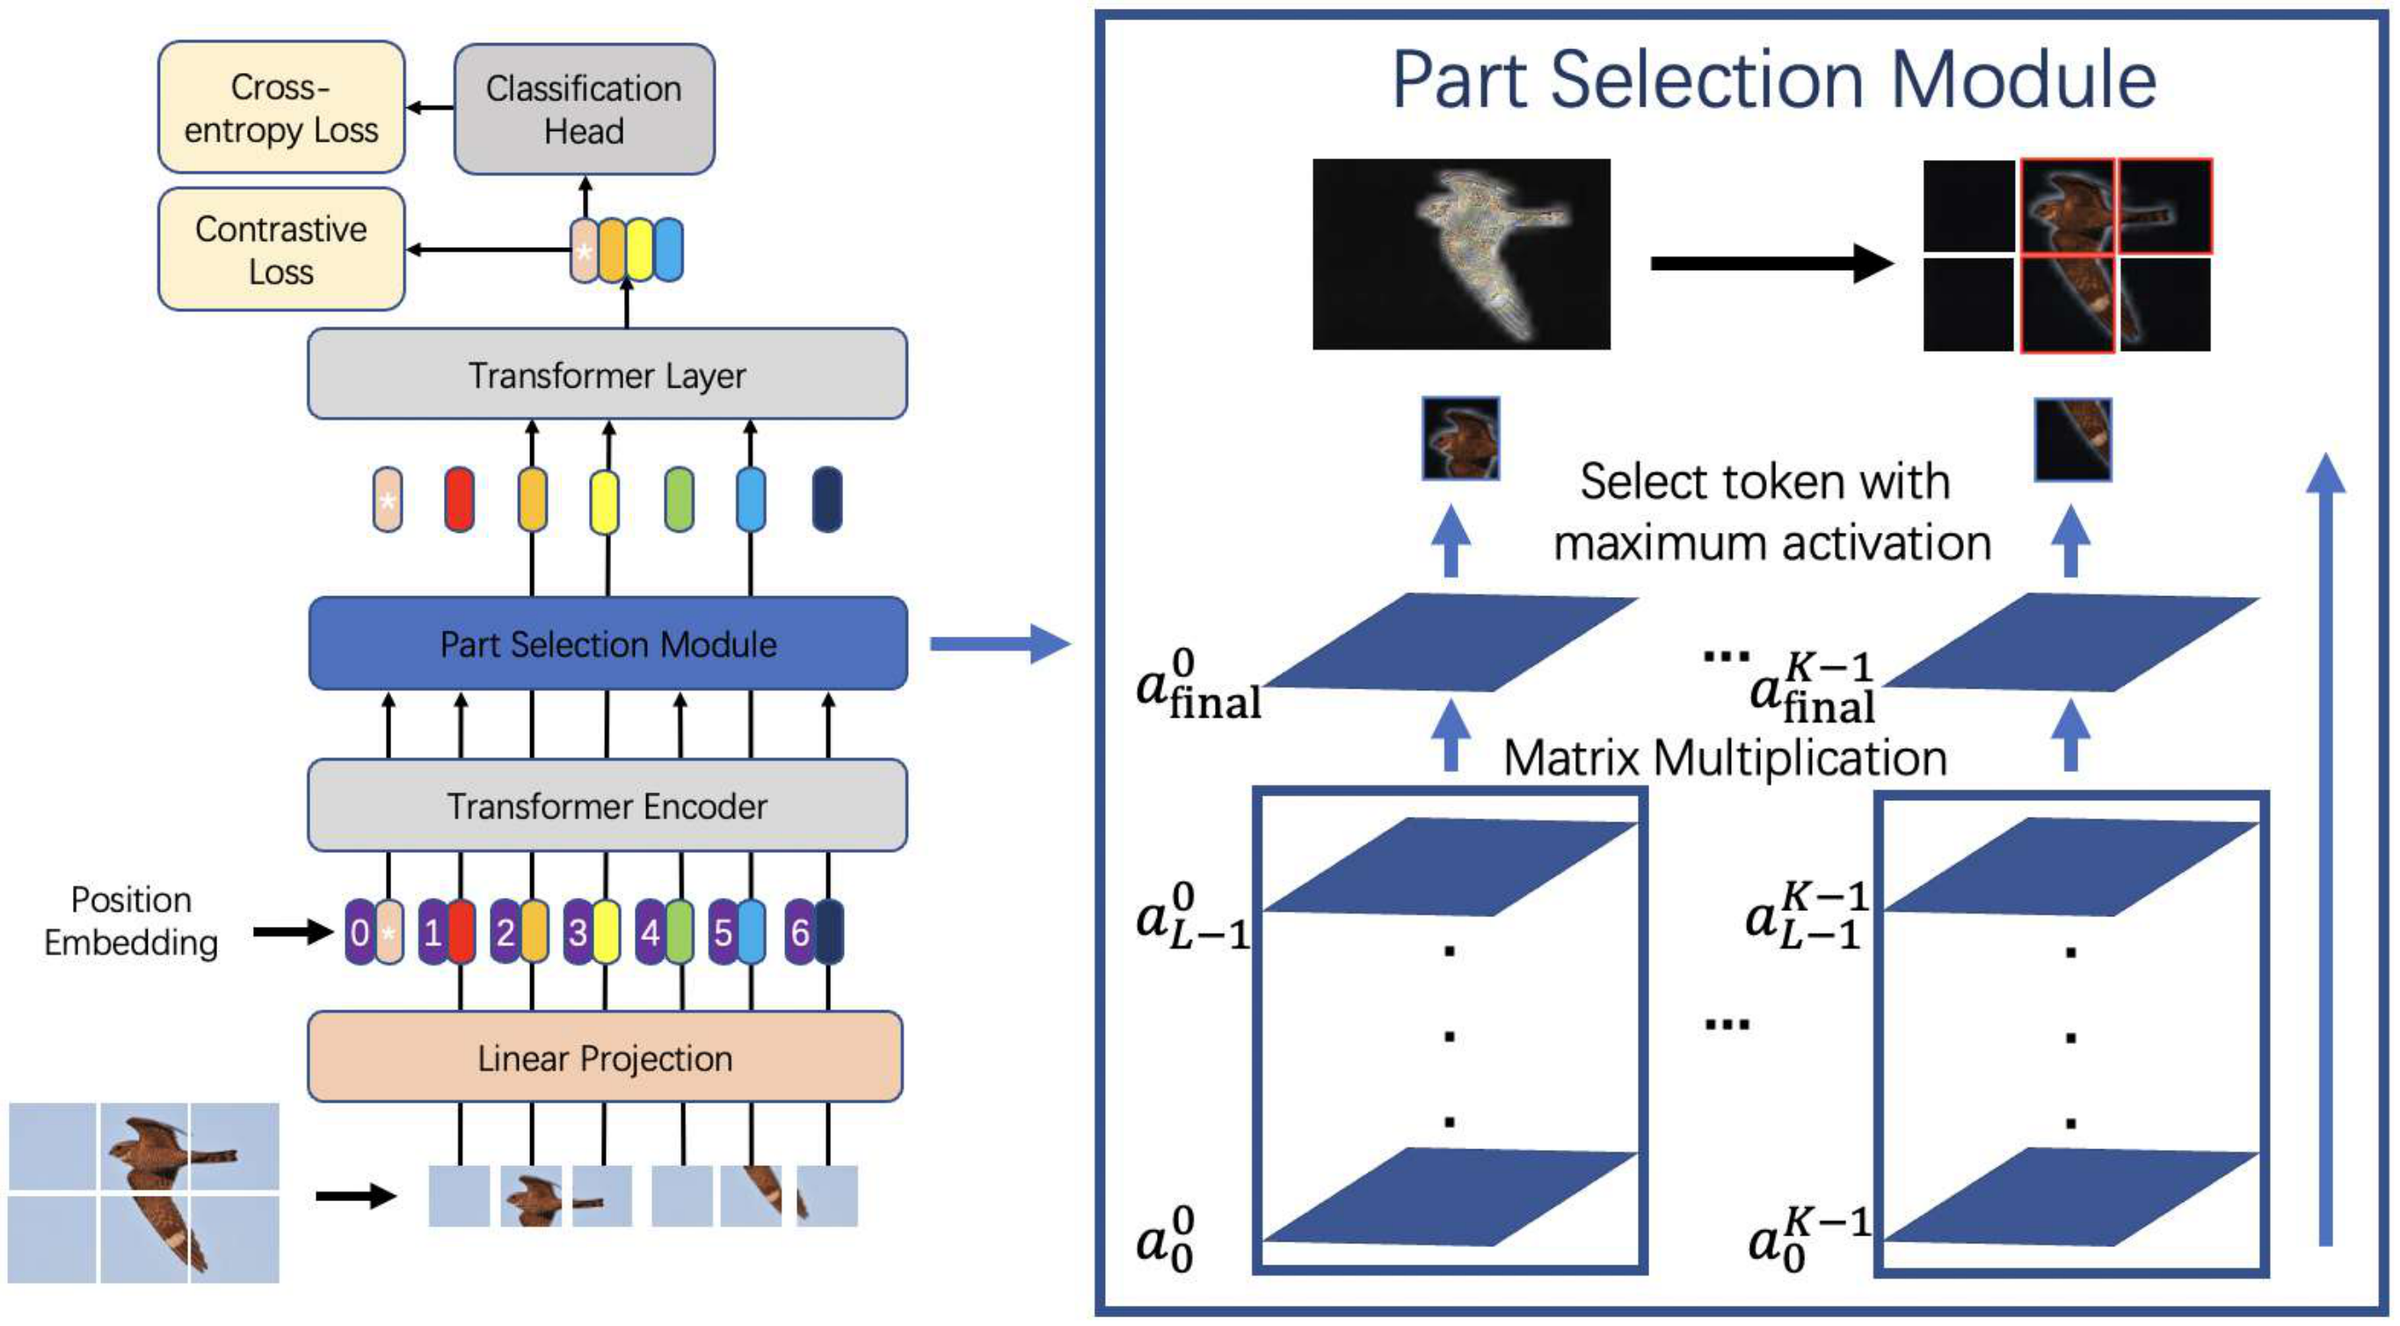
\includegraphics[width=\linewidth,height=0.56\textheight,keepaspectratio]{images/image-recognition/transfg_fig2_framework.png}\\[0.2em]
      {\scriptsize The figure draws a non-overlapping split. He et al., ``TransFG: A Transformer Architecture for Fine-grained Recognition,'' AAAI 2022, \href{https://arxiv.org/abs/2103.07976v5}{arXiv:2103.07976v5}, Figure~2; results from Tables 1 and 5--7.\par}
  \end{columns}
\end{frame}

\begin{frame}{Frozen Foundation Features on Fine-Grained Data}
  \begin{columns}[T,onlytextwidth]
    \column{0.54\textwidth}
      \centering
      {\scriptsize Linear probes on frozen features (covered earlier), accuracy \% (mean per class for Aircraft). Cars, Aircraft, CUB: logistic regression (Table~8); iNat21: trained linear layer (Table~7).\par}
      \vspace{0.2em}
      {\scriptsize\setlength{\tabcolsep}{4pt}
      \begin{tabular}{l r r r r}
        \toprule
        \textbf{ViT features} & \textbf{Cars} & \textbf{Aircraft} & \textbf{CUB} & \textbf{iNat21} \\
        \midrule
        MAE H/14 & 56.1 & 63.4 & 57.2 & 32.3 \\
        DINO B/8 & 76.6 & 70.6 & 81.7 & 68.3 \\
        iBOT L/16 & 71.8 & 72.4 & 82.1 & 74.6 \\
        OpenCLIP G/14 & \textbf{96.1} & 80.2 & 89.9 & 76.0 \\
        DINOv2 g/14 & 91.4 & \textbf{87.2} & \textbf{91.6} & \textbf{85.7} \\
        \bottomrule
      \end{tabular}\par}
      \vspace{0.3em}
      \begin{itemize}\scriptsize\itemsep0.25em
        \item DINOv2 leads the best earlier self-supervised features by 14.8 points on both Cars and Aircraft, and beats text-supervised OpenCLIP on Aircraft and CUB.
        \item \textbf{Caveat}: LVD-142M, DINOv2's curated training set (covered earlier), includes 1M web images retrieved near the training split of each of Cars, Aircraft and CUB. iNaturalist was left out of that retrieval, and there DINOv2 leads OpenCLIP by 9.7 points.
      \end{itemize}
    \column{0.44\textwidth}
      \centering
      {\scriptsize CLIP ViT-L/14@336px, accuracy \% (mean per class for Aircraft, Pets, Flowers)\par}
      \vspace{0.2em}
      {\scriptsize\setlength{\tabcolsep}{4pt}
      \begin{tabular}{l r r}
        \toprule
        \textbf{Dataset} & \textbf{Zero-shot} & \textbf{Probe} \\
        \midrule
        FGVC-Aircraft & 37.2 & 71.6 \\
        Birdsnap & 49.5 & 79.9 \\
        Flowers102 & 78.3 & 99.2 \\
        Stanford Cars & 78.8 & 91.5 \\
        Oxford Pets & 93.5 & 95.1 \\
        \bottomrule
      \end{tabular}\par}
      \vspace{0.3em}
      \begin{itemize}\scriptsize\itemsep0.25em
        \item The probe reads CLIP's image features before the final projection, and zero-shot CLIP is also a linear classifier on them, so the fine-grained weakness (covered earlier) comes from the class weights: weights from class-name prompts against weights fitted to labelled images. The gap is 34.4 points on Aircraft and 1.6 on Pets.
        \item Across CLIP's evaluation datasets, zero-shot accuracy is mostly 10--25 points below the linear probe.
      \end{itemize}
  \end{columns}
  \vspace{0.1em}
  {\scriptsize Oquab et al., ``DINOv2: Learning Robust Visual Features without Supervision,'' TMLR 2024, \href{https://arxiv.org/abs/2304.07193v2}{arXiv:2304.07193v2}, Tables 7, 8, 15 and 18; Radford et al., ``Learning Transferable Visual Models From Natural Language Supervision,'' ICML 2021, \href{https://arxiv.org/abs/2103.00020v1}{arXiv:2103.00020v1}, Tables 10--11 and Figure~8.\par}
\end{frame}

\begin{frame}{BioCLIP: The Taxonomy as Text Supervision}
  \centering
  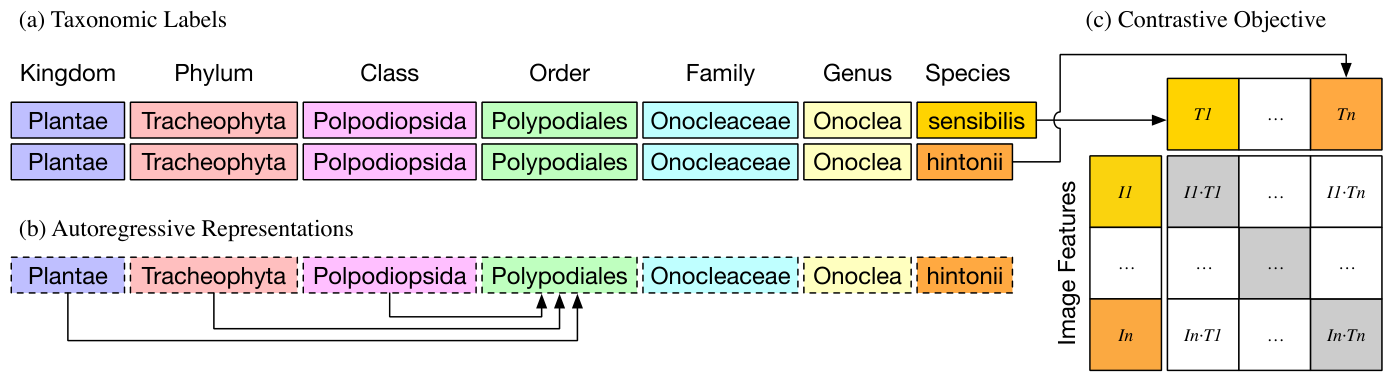
\includegraphics[width=\textwidth,height=0.32\textheight,keepaspectratio]{images/image-recognition/bioclip_fig1abc_taxonomic_labels.png}\\[0.15em]
  {\scriptsize Stevens et al., ``BioCLIP: A Vision Foundation Model for the Tree of Life,'' CVPR 2024, \href{https://arxiv.org/abs/2311.18803v3}{arXiv:2311.18803v3}, Figure~1(a)--(c); Tables 1, 3 and 5.\par}
  \vspace{0.3em}
  \begin{columns}[T,onlytextwidth]
    \column{0.50\textwidth}
      \begin{itemize}\scriptsize\itemsep0.3em
        \item \textbf{TreeOfLife-10M}: 10.4M images of 454,103 taxa, merged from iNat21 (2.7M), BIOSCAN-1M laboratory photos of insects (1.1M) and the Encyclopedia of Life (6.6M), relabelled into one taxonomy.
        \item \textbf{Taxonomic name}: the seven ranks from kingdom to species joined into one string. The text encoder is causal (each token attends only to earlier tokens), so each rank is encoded given the ranks above it (panel b), and an unseen species can reuse what was learned for its genus and family.
        \item \textbf{Training}: the CLIP objective (covered earlier), starting from OpenAI's CLIP ViT-B/16; 100 epochs at batch size 32,768.
      \end{itemize}
    \column{0.48\textwidth}
      \begin{itemize}\scriptsize\itemsep0.3em
        \item \textbf{Text types}: common (black-billed magpie), scientific (\textit{Pica hudsonia}), taxonomic (Animalia Chordata Aves Passeriformes Corvidae \textit{Pica hudsonia}), and combinations such as taxonomic plus common name.
        \item \textbf{Mixed text types}: each training step pairs an image with one of its text types drawn at random, so other name types can be used at test time.
        \item On 400 at-risk species excluded from training, a model trained on scientific names alone scores 22.3\% with scientific-name prompts and 4.5\% with taxonomic ones; mixed training scores 24.9--30.9\% for every prompt type (1M-image ablation).
      \end{itemize}
  \end{columns}
\end{frame}

\begin{frame}{BioCLIP Results and Scaling to BioCLIP 2}
  \begin{columns}[T,onlytextwidth]
    \column{0.52\textwidth}
      \centering
      {\scriptsize Mean top-1 \% over 10 biology tasks, all ViT-B/16 (Stevens et al., Table~4)\par}
      \vspace{0.2em}
      {\scriptsize\setlength{\tabcolsep}{4pt}
      \begin{tabular}{l r r r}
        \toprule
        \textbf{Model} & \textbf{Zero-shot} & \textbf{1-shot} & \textbf{5-shot} \\
        \midrule
        CLIP & 21.9 & 33.6 & 51.5 \\
        OpenCLIP & 20.4 & 36.7 & 55.9 \\
        DINO (image only) & n/a & 36.2 & 55.4 \\
        BioCLIP, iNat21 data only & 31.7 & 47.5 & 65.1 \\
        BioCLIP & \textbf{39.4} & \textbf{50.3} & \textbf{68.8} \\
        \bottomrule
      \end{tabular}\par}
      \vspace{0.3em}
      \begin{itemize}\scriptsize\itemsep0.3em
        \item \textbf{$k$-shot}: each class is the mean of its $k$ image embeddings, and a test image takes the class with the nearest mean. For zero-shot prompts, CLIP and OpenCLIP get common names, their best name type.
        \item Trained on iNat21 alone (2.7M images, 10,000 species), the same recipe reaches 31.7 zero-shot; the larger and broader TreeOfLife-10M adds the remaining 7.7 points.
      \end{itemize}
    \column{0.46\textwidth}
      \begin{itemize}\scriptsize\itemsep0.25em
        \item \textbf{BioCLIP 2} scales the recipe: TreeOfLife-200M (214M images, 952K taxa), a ViT-L/14 encoder, and 26M replayed LAION-2B image-text pairs.
        \item Mean zero-shot accuracy over its 10 species tasks rises from 37.6 (BioCLIP) to 55.6.
        \item With no trait labels, the embeddings order Darwin's finches by beak size (below) and keep life stage and sex orthogonal to the species differences.
      \end{itemize}
      \centering
      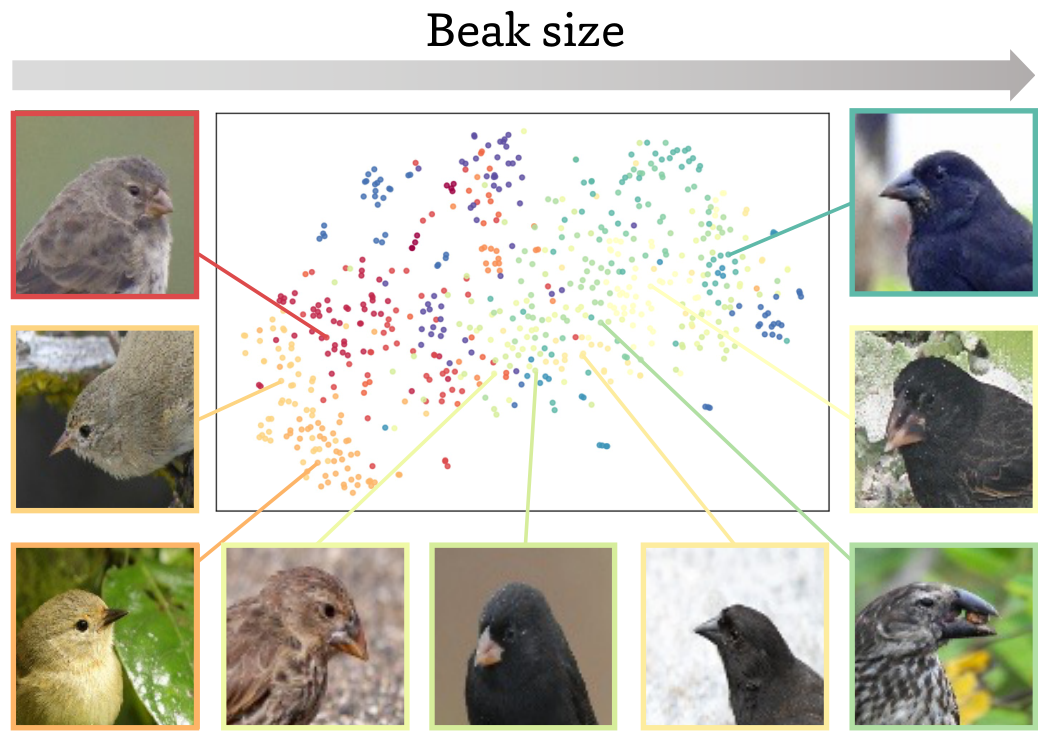
\includegraphics[width=\linewidth,height=0.30\textheight,keepaspectratio]{images/image-recognition/bioclip2_fig1_finch_beak_size.png}\\[0.2em]
      {\scriptsize Gu et al., ``BioCLIP 2: Emergent Properties from Scaling Hierarchical Contrastive Learning,'' NeurIPS 2025, \href{https://arxiv.org/abs/2505.23883v2}{arXiv:2505.23883v2}, Figure~1 (left); Table~1.\par}
  \end{columns}
\end{frame}

\begin{frame}{Vision-Language Assistants as Classifiers}
  \begin{columns}[T,onlytextwidth]
    \column{0.52\textwidth}
      \begin{itemize}\scriptsize\itemsep0.3em
        \item Vision-language models (VLMs, covered earlier) such as LLaVA-1.5 feed image-encoder outputs through a small projector into a language model; LLaVA-1.5 uses CLIP-L (CLIP ViT-L/14 at 336 pixels). With all class names in the prompt, an answer counts as correct if it contains the true label.
        \item \textbf{Gap}: on Stanford Cars every VLM tested trails CLIP-L used zero-shot. LLaVA-1.5-7B scores 10.2\% on Flowers102, where its own encoder scores 76.0\%.
        \item \textbf{The information is kept}: a linear probe on LLaVA-1.5-7B's last-layer features reaches 82.8\% on Cars, and training only the projector to generate the label text reaches 90.4\% (CLIP-L probe: 91.5\%).
        \item \textbf{Data decides}: ImageNet classes named fewer than 10 times in LLaVA's training data score 3.0\%, classes named over 10,000 times 82.7\% (rank correlation 0.76).
        \item \textbf{Fix}: adding ImageNet's 1.28M labelled images to LLaVA's 665K instruction-tuning examples lifts ImageNet accuracy from 22.8\% to 84.4\% and ImageWikiQA (questions that need the object's class) from 38.0\% to 49.8\%. ImageNet data alone drops ImageWikiQA to 30.6\%.
      \end{itemize}
    \column{0.46\textwidth}
      \centering
      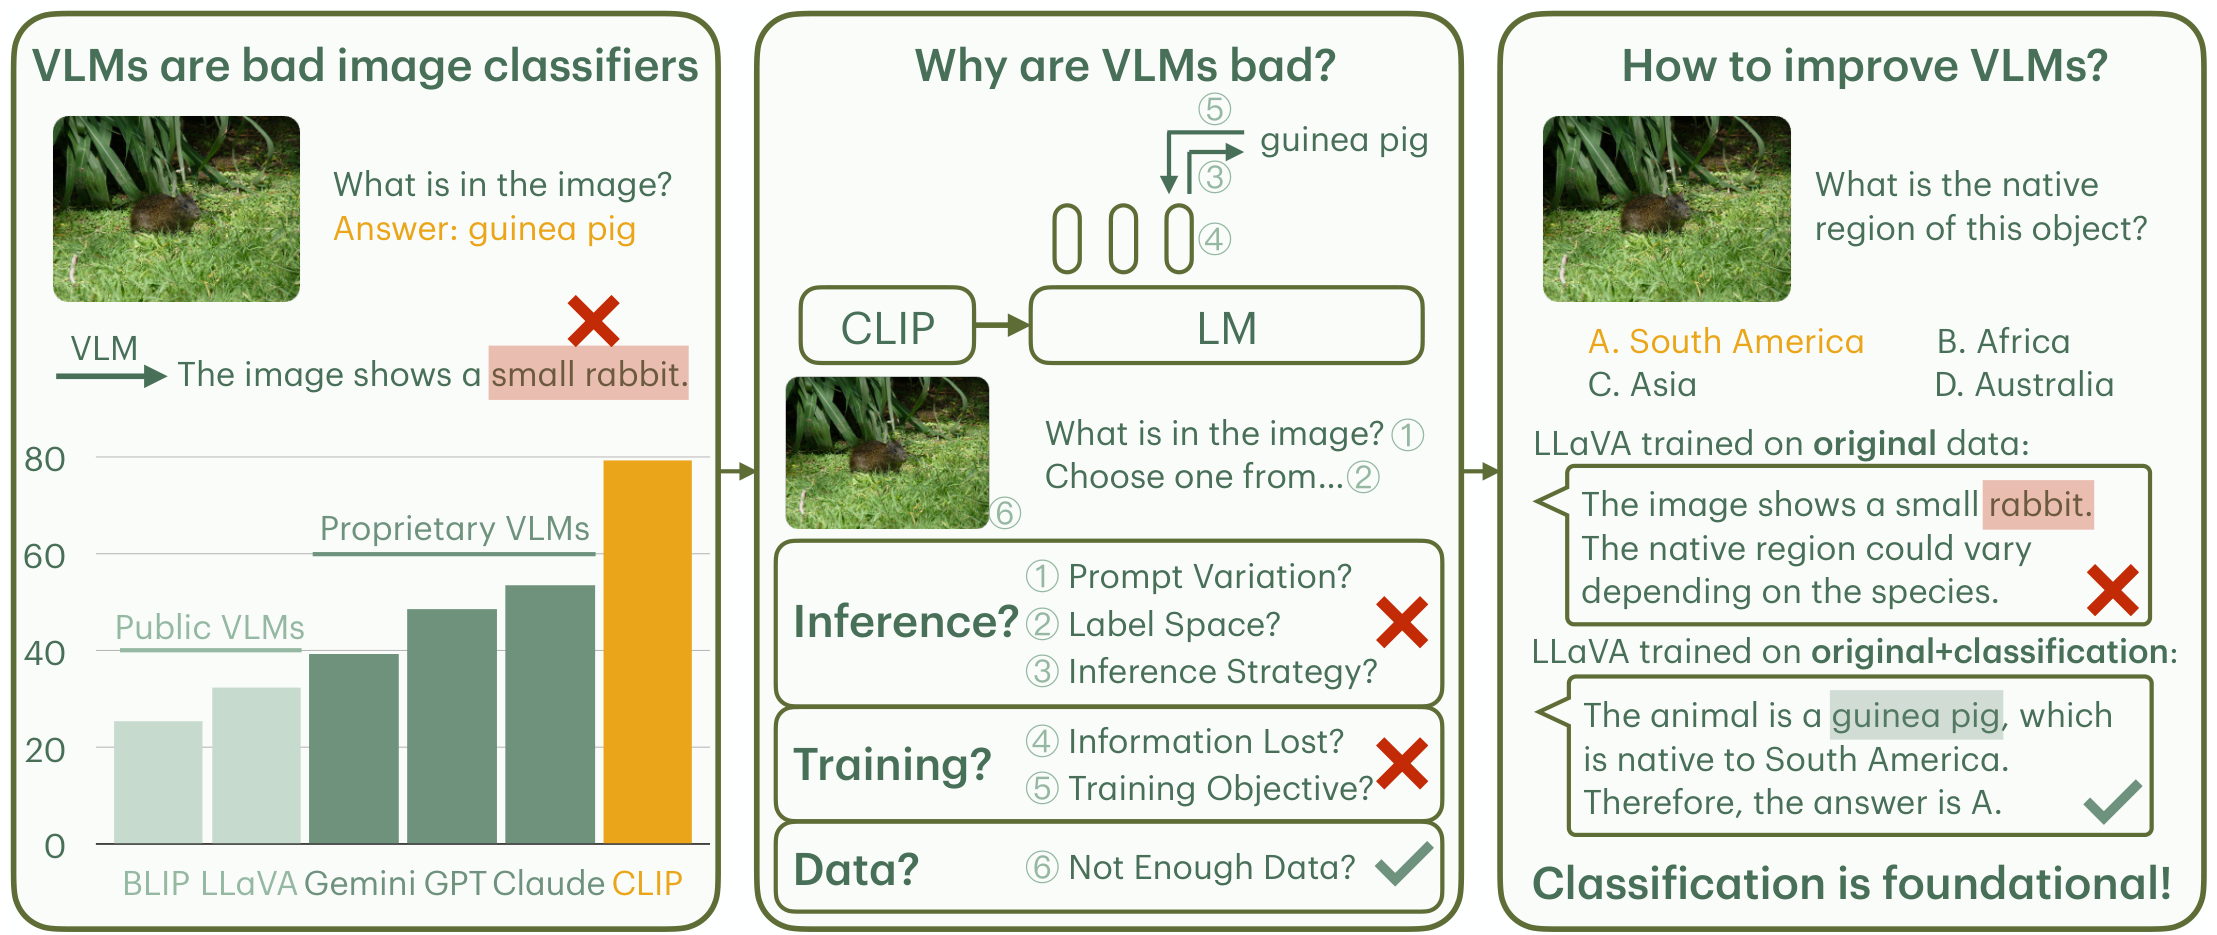
\includegraphics[width=\linewidth,height=0.30\textheight,keepaspectratio]{images/image-recognition/vlmcls_fig1_overview.png}\\[0.2em]
      {\scriptsize Zhang et al., ``Why are Visually-Grounded Language Models Bad at Image Classification?'' NeurIPS 2024, \href{https://arxiv.org/abs/2405.18415v2}{arXiv:2405.18415v2}, Figure~1; Tables 1, 3, 5 and Sec.~3.3.\par}
      \vspace{0.4em}
      {\scriptsize Accuracy (\%) with all class names in the prompt (Table~1)\par}
      \vspace{0.2em}
      {\scriptsize\setlength{\tabcolsep}{4pt}
      \begin{tabular}{l r r r}
        \toprule
        \textbf{Model} & \textbf{ImageNet} & \textbf{Flowers102} & \textbf{Cars} \\
        \midrule
        LLaVA-1.5-7B & n/a & 10.2 & 0.0 \\
        Claude 3 Opus & 51.1 & 58.3 & 45.1 \\
        Gemini Pro Vision & 56.0 & 62.0 & 66.6 \\
        GPT-4 Turbo & 60.6 & 79.9 & 58.2 \\
        CLIP-L, zero-shot & 74.8 & 76.0 & 77.5 \\
        \bottomrule
      \end{tabular}\par}
      {\scriptsize n/a: 1,000 class names do not fit LLaVA's 4K-token context.\par}
  \end{columns}
\end{frame}
